\documentclass[11pt]{article}
\usepackage[spanish]{babel}


%%%%%%%%%%%%%%%%%%%%%%%%%%%%%%%%%%
%%%%%%%%%%%%%%%%%%%%%%%%%%%%%   %%
%%        Datos Trabajo     %%  %%
%%%%%%%%%%%%%%%%%%%%%%%%%%%%%%%%%%
\newcommand{\titulo}[0]{Reto 3. Mis finanzas}
\newcommand{\materia}[0]{Finanzas Personales v1}


%%%%%%%%%%%%%%%%%%%%%%%%%%%%%%%%%%
%%%%%%%%%%%%%%%%%%%%%%%%%%%%%%%%%%
\usepackage{amssymb}
\usepackage{enumerate}
\usepackage{geometry}
\usepackage{mathtools}
\usepackage{multicol}
\usepackage{soul}

\usepackage{graphicx}
	\graphicspath{ {assets/} }

\usepackage{hyperref}
	\hypersetup{
			pdftex,
		        pdfauthor={bench},
		        pdftitle={...},
		        pdfsubject={...},
		        pdfkeywords={UVEG},
		        pdfproducer={Latex with hyperref, Ubuntu},
		        pdfcreator={pdflatex, or other tool},
			colorlinks=true,
				linkcolor=[rgb]{0,0,0.45},
				urlcolor=cyan,
				filecolor=green,
				citecolor=blue}

%%%%%%%%%%%%%%%%%%%%%%%%%%%%%%%%%%
%%%%%%%%%%%%%%%%%%%%%%%%%%%%%%%%%%

\title{\titulo}

\author{ Universidad Virtual del Estado de Guanajuato \textbf{UVEG} \\ 
\materia \\ Benjamín Rivera \\ 19015478 }
\date{\textit{Fecha de entrega:} \today}


%%%%%%%%%%%%%%%%%%%%%%%%%%%%%
%%        Documento         %%
%%%%%%%%%%%%%%%%%%%%%%%%%%%%%%%
\begin{document}
	\maketitle
	
	\begin{figure}[htp]
		\centering
		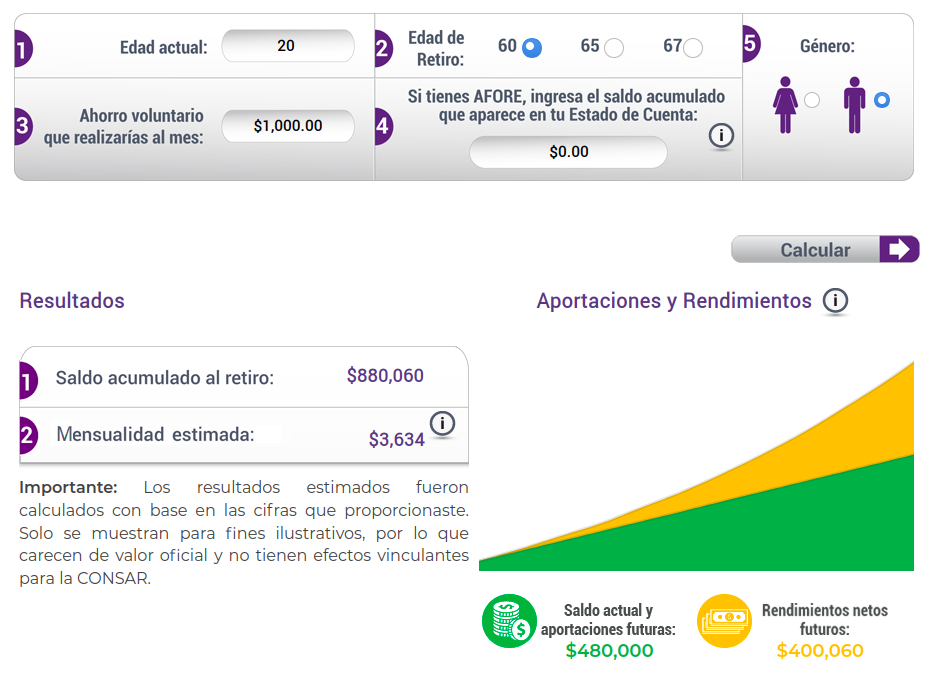
\includegraphics[width=\textwidth]{assets/R3_U1-aprox_afore.png}
		\caption{Calculo de posible pension.}
		\label{}
	\end{figure}
	
	\subsubsection*{¿El resultado obtenido te parece suficiente para poder cubrir una  vida  digna?}
	
	\par A decir verdad mi vida laboral aún no ha empezado, por el momento me he dedicado completamente al estudio y he dejado un poco de lado cosas como mi pensión y la época de mi retiro. Después de ver esta gráfica me doy cuenta de que se me empieza a agotar el tiempo para poder conseguir una pensión digna. Por otro lado, me parece una buena opción considerar los \textit{Planes Personales para el Retiro}, que son otro instrumento financiero que pueden apoyarme a tener un retiro más digno.
	\par En primera instancia veo que lo ideal sería aportar mas a mi ahorro de lo que considere en la captura que adjunto como evidencia. Haciendo pruebas veo que no es necesario aumentarlo demasiado (me imagino a que estos cambios se muestran por la magia de los intereses compuestos), si se hace un ahorro voluntario de $\$2,000$, se llega a una cifra un poco más digna de $\$7,000$ mensuales. Con lo cual, posiblemente, se pueda vivir mejor. Aunque claramente ya no es una cifra de la cual se pueda despreciar directamente.
	\par Definitivamente estos movimientos están limitados a los conservadurismos que se mantienen en los afores públicos (que los considero aceptables por las responsabilidades que tienen). Esto se puede mejorar con PPR's privados, que pueden ser un poco más agresivos para tratar de conseguir mejores rendimientos para sus beneficiaros.
	
	\begin{figure}[htp]
		\centering
		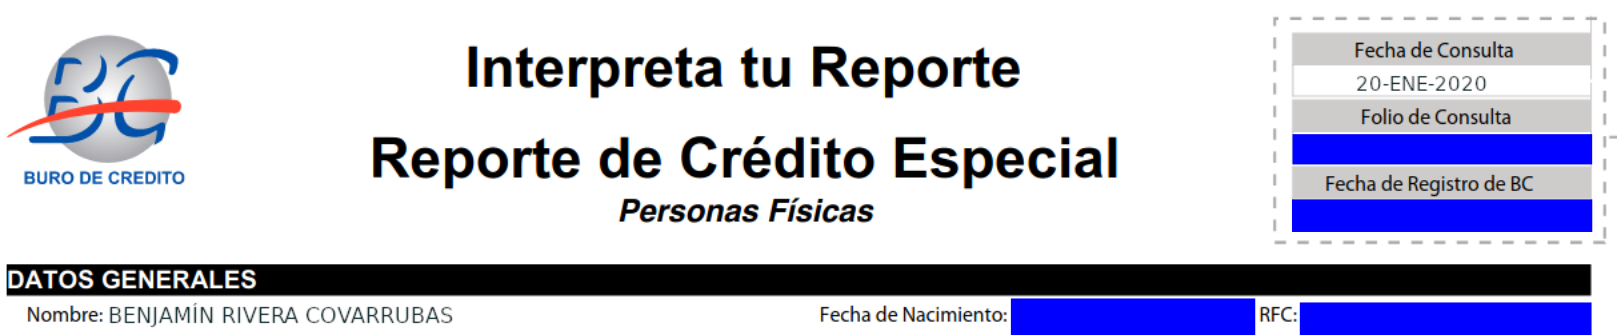
\includegraphics[width=\textwidth]{assets/R3_U1-reporte_buro2.png}
		\caption{Ejemplo de reporte de buro de credito}
		\label{}
	\end{figure}
	
	\par De manera parecida a la reflexión anterior, en este momento de la vida, aún no tengo el nivel de responsabilidades que me hayan llevado a pedir alguna clase de crédito. Además de que todo lo que he tenido que adquirir lo he hecho mediante la modalidad de contado. Por lo mismo mi historial crediticio, y por lo tanto mi buró de crédito, están limpios.
	\par La principal desventaja que le veo a esto es que no puedo acceder a instrumentos crediticios complejos y con más ventajas. De manera que, fuera de las tarjetas de crédito garantizadas, todos los demás instrumentos están fuera de mi alcance por falta de historial.
	\par Esto no implica que desprecie, o algo parecido, a los créditos. Creo que son herramientas financieras que, usadas de manera responsable y cuidando mi salud financiera, pueden ayudarme a conseguir de manera más holgada ciertas metas y objetivos financieros. Además de que instrumentos crediticios como las tarjetas de crédito también pueden ofrecer otros beneficios por parte delos bancos que lo ofrezcan.
	
	\par En general ahora noto que, a menos de que se tenga la oportunidad de trabajar (legalmente, porque luego los estudiantes no nos aceptan en trabajos regulados) y estudiar al mismo tiempo, toda nuestra época de estudio es un tiempo que tenemos vacía financieramente hablando. Esto es algo que me gustaría poder solucionar pronto, para poder llegar a un punto de buena salud financiera pronto.



%%%%%%%%%%%%%%%%%%%%%%%%%%%%%%%%
%%         Bibliografia        %%
%%%%%%%%%%%%%%%%%%%%%%%%%%%%%%%%%%

	\begin{thebibliography}{X}
	
		\bibitem{1} Localiza tu AFORE. (s/f). Recuperado el 20 de enero de 2021, \url{de https://www.e-sar.com.mx/PortalEsar//public/consultaAforeInicio.do}
		
		\bibitem{2} Reporte de Crédito Especial. (s/f). Recuperado el 20 de enero de 2021, de \url{https://wbc1.burodecredito.com.mx:543/RceOnline/autorizacion.faces}

		\bibitem{3}Retiro, C. N. del S. de A. para el. (s/f). Calculadoras de Ahorro y Retiro. gob.mx. Recuperado el 20 de enero de 2021, de \url{http://www.gob.mx/consar/acciones-y-programas/calculadoras-de-ahorro-y-retiro?idiom=es}
	\end{thebibliography}

\end{document}